%%==================================================
%% chapter02.tex for BIT Master Thesis
%% modified by liu xiahua
%% version: 0.1
%% last update: May 20th, 2018
%%==================================================

\chapter{参数匹配}
\label{chap:calculation}

电池系统参数匹配是在设计电池箱中的重要环节,电池系统的参数需要提前通过计算或者实验方法确定。相比传统汽车使用内燃机作为动力转换装置,电动汽车内要完成“化学能-电能-机械能”的两个能量转换过程,而这两个转换过程分别在电池系统和车载电动机内完成,故电动车的动力性能不仅仅受到电动机的影响,还和车载的电池系统有密切的关系。

理论研究证明,电池系统的参数与车辆参数的匹配程度可以直接影响电池系统的寿命和车辆的使用性能。电池箱参数不合理的过低设计会导致电池发生过放现象,产生危险,或者车辆的驱动性能受到影响;而对于电池箱的参数设计超过车辆的使用需求又会导致车辆本身重量过大,滚动阻力增加从而导致效率下降,和车辆制造成本的提高。本文将会对大众某型号的电动汽车进行电池系统的参数匹配,在匹配过程中完成理论计算和软件仿真的两个步骤,最后完成电池系统参数的确定并给出系统参数。

目前市面上已经存在有许多不同品牌的电动车型和混合动力车型,如日产 LEAF,特斯拉 Model S 和雪佛兰 Volt 宝马 i3 等。可以看到,由于锂电池的优越性能 \cite{王艺颖2017锂电池的发展现状及与镍氢电池的比较},越来越多的车型在逐渐的抛弃传统的镍氢电池技术,转而研究和使用性能更加优异的锂离子电池系统。根据各个车辆制造商拥有的不同的车辆电池系统电池摆放策略的专利细节信息,大多数的电池系统中的电池摆放结构是:电池单体首先以并联的形式组成一个个电池模块,然后再以串联的形式将一个个电池模块组成一个整体的电池组,又称电池包。

最终的电池包应该符合相关的车辆平台要求,例如其总能量能够满足车辆一定的续航里程,功率能够满足日常使用的爬坡和起步要求,电池包的开路电压也应该在一个合理的区间之内。基于此,本文根据某实际车型的相关物理参数,对该车型的电池系统参数进行了设计,并在参数设计完成时,使用了仿真软件 AVL Cruise,将设计的电池参数输入该软件,仿真该电池系统在实际车上的性能表现,验证设计的可行性。

\section{已给定的匹配信息}

\subsection{电池单体参数}
因为锂离子电池的优秀性能表现 \cite{赵金龙2014增程式电动汽车动力系统参数匹配及能量管理策略研究},在本文设计中,使用的电池型号为天津力神电池股份有限公司生产的 LP2714897 锂离子电池。该电池的标称电压为3.65 V,标称容量为 37.0 Ah,电池相关信息如表 \ref{tab:cell} 所示。

\begin{table}
	\centering
	\caption{天津力神动力型锂电池型号信息} \label{tab:cell}
	\begin{tabular*}{0.9\textwidth}{@{\extracolsep{\fill}}cc}
		\toprule
		项目			&规格		 \\
		\midrule
		电池型号	     &LP2714897  \\
		标称容量		 &37.0 Ah	 \\
		标称电压	     &3.65 V     \\
        直流内阻      	 &≤1.8 m$\Omega$ (10 s,1 C,50\% SOC) \\
        最大放电电流     &6 C (连续);10 C (10 s)\\
		\bottomrule
	\end{tabular*}
\end{table}

\subsection{整车数据}
本文设计以及计算的对象为现有的大众某电动汽车车型,该车的整车信息如表 \ref{tab:vehi} 所示。本文所匹配车辆的目标指标如图 \ref{tab:target} 所示。

\begin{table}
	\centering
	\caption{大众 e-Golf 车型信息} \label{tab:vehi}
	\begin{tabular*}{0.9\textwidth}{@{\extracolsep{\fill}}cc}
		\toprule
		参数			&数值		 \\
		\midrule
		整备质量/kg	     &1540  \\
		满载质量/kg		 &2020  \\
		迎风面积/m$^2$   &2.6666\\
		空气阻力系数     &0.35  \\
		滚动阻力系数     &0.014 \\
        最高车速/(km/h)  &150   \\
		\bottomrule
	\end{tabular*}
\end{table}

\begin{table}
	\centering
	\caption{车辆的动力性设计指标} \label{tab:target}
	\begin{tabular*}{0.9\textwidth}{@{\extracolsep{\fill}}cc}
		\toprule
		参数			&数值		 \\
		\midrule
		最高车速/(km/h)  & $\geq150 $  \\
		20 km/h 最大爬坡度/\% & $\geq 30$ \\
		0$\sim$50 km/h 加速时间 /(s) & $\leq 15$ \\
		\bottomrule
	\end{tabular*}
\end{table}

\section{电池参数理论计算}
电池系统的主要设计参数在本文中被分为两方面,第一个方面是电池箱的功率性能应该能够满足车辆的某些行驶需求,第二个方面是电池箱的容量能够支持车辆行驶一定的里程。这两方面是电池箱设计中最关键的两个参数,电池箱设计过程必须要达到功率指标和容量指标,否则在安装到车辆上后,电池箱不足以满足车辆正常行驶的功能。

\subsection{电池系统额定功率计算}
电池系统的功率与车辆的动力性能息息相关。虽然电动车辆是直接通过电动机驱动车辆前进的,但是在能量转换链上,电池箱是电动汽车电动机的能量来源,一旦电池箱不能够提供给电动机足够的功率,电机将无法输出足够的动力给车轮。对于电动车的电池系统的功率匹配,可以通过车辆的三个行驶性能入手,分别为车辆的最高车速、车辆的爬坡度,以及车辆的加速性能 \cite{phev-zongshu}。

\subsubsection{最高车速性能匹配}
在前面的部分,本文给出了车辆设计最终的性能指标,车辆在极速状态下,应该能够达到速度超过 150 km/h 的性能,车辆的最高车速性能与电池箱的额定功率有着密切的关系,根据功率的计算方程 \cite{刘昭度2012汽车学},车辆的最高车速和车辆所需的额定功率有以下关系:

\begin{equation}
\eta_T\eta_EP_{e1} = F_T v_{max}
\end{equation}

另一方面,车辆的行驶方程如下所示:

\begin{equation}
	\label{equ:powerequ}
F_T = F_f+F_w+F_i+F_j	
\end{equation}

式中,$\eta_T$为机械效率,在这里取一般情况下的数据,$\eta_T = 96\%$,$\eta_E$ 为驱动电机的工作效率,在这里根据车型搭配的电动机万有特性曲线,取平均值 $\eta_E = 85\%$ 。$P_{e1}$ 为电池额定功率,$v_{max}$ 为最大车速,$F_T$ 为达到功率平衡时的驱动力。$F_f$ 为汽车的滚动阻力,$F_w$ 为汽车的空气阻力,$F_i$ 为汽车的坡道阻力,$F_j$ 为汽车的加速阻力。在这里,道路情况默认为平直道路,车辆为匀速行驶,故 $F_i = F_j = 0$。

得到:
\begin{equation}
\label{equ:zuli}
P_{e1} = v_{max} (Gf+\frac{C_DA}{21.15}v_{max}^2)/(\eta_T\eta_E)
\end{equation}

式中,$G$ 为所匹配车辆的整备重量,$f$ 为路面的滚动摩擦阻力系数,$C_D$ 为所匹配车辆的空气阻力系数,$A$ 为该车型的迎风面积。

\begin{figure}
	\centering
	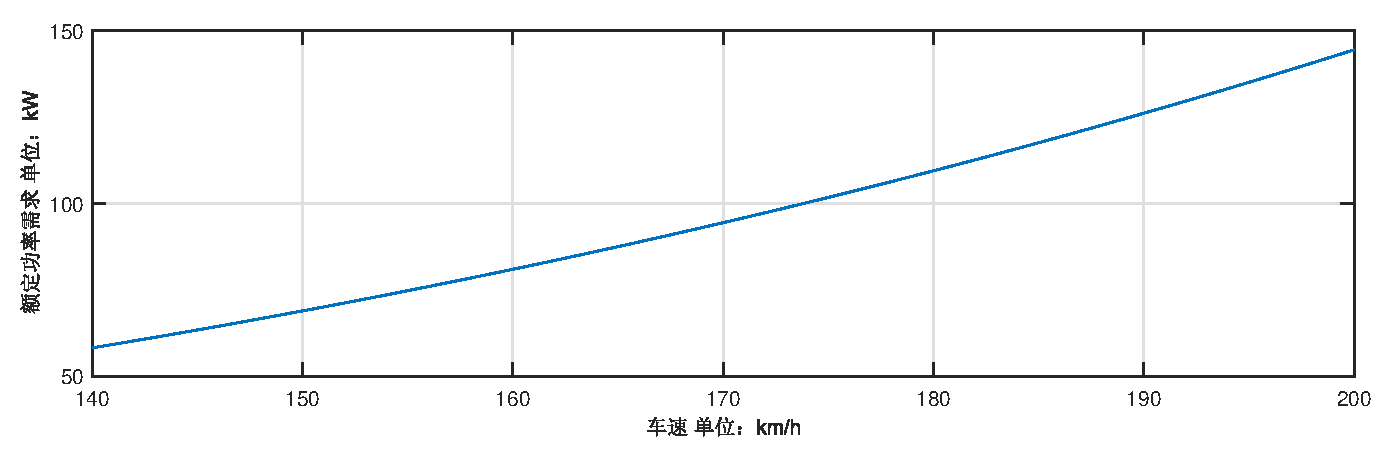
\includegraphics[width=0.9\textwidth]{figures/pe.eps}
	\caption{额定功率与最高车速图}\label{fig:pe}
\end{figure}

带入数据,计算得到的结果如图 \ref{fig:pe},电池额定功率取 $P_{e1}=68.89 kW$。

\subsubsection{爬坡度性能匹配}

当驾驶员驾驶车辆通过坡道路面的时候,车辆需要输出较大的扭矩,在爬坡状态下,车辆的行驶速度应该也能够得到保证,在表 \ref{tab:target} 中可以看到本文设计目标是车辆能够以 20km/h 的速度越过 30$^\circ$ 的坡道。同理,根据车辆平衡方程,爬坡度参数匹配的计算的公式如下所示:

\begin{equation}
	P_{e2} = v_{1} (G\sin\alpha_{max}+Gf\cos\alpha_{max}+\frac{C_DA}{21.15}v_{1}^2)/(\eta_T\eta_E)
\end{equation}

式中,$\eta_T$为机械效率,在这里取一般情况下的数据,$\eta_T = 96\%$,$\eta_E$ 为驱动电机的工作效率,在这里根据车型搭配的电动机万有特性曲线,取平均值 $\eta_E = 85\%$ 。$P_{e2}$ 为电池爬坡所需要的额定功率,$v_{1}$ 为爬坡时的车速,$f$ 为路面的滚动摩擦阻力系数,$\alpha$ 为本文预设的爬坡角度,在这里 $\alpha_{max}=\tan^{-1}(30\%)\approx 16.7^\circ$。
可以得到的额定功率应当满足条件:\ $P_{e2}= 40.53 kW$。

\subsubsection{加速性能匹配}
电动车辆起步的时候,车辆的扭矩需要满足一定值,否则车辆的加速性能较弱。电池箱的输出功率应该能够使得车辆的加速度满足表 \ref{tab:target} 中相关的要求。涉及到加速度的计算比较复杂,在这里本文假设车辆是按照恒功率 $P_{e3}$ 的状态进行起步加速的。

在匹配电池箱的加速性能参数时,应当把汽车的行驶方程改写,首先计算车辆的动力因数:

\begin{equation}
\begin{aligned}
	\label{equ:jiasu}
	D=\frac{F_t-F_w}{G}&=\frac{\frac{P_{e3}}{v\eta_T\eta_E}-\frac{C_DA}{21.15}v^2}{2020\times 9.8}\\
	\frac{\mathrm{d}v}{\mathrm{d}t}&=\frac{g}{\delta}(D-f)
\end{aligned}
\end{equation}

式中,$D$ 为匹配参数的车辆在加速时的动力因数,$f$ 为滚动阻力系数,$\delta$ 为该车辆的轿车旋转质量换算系数,计算匹配车辆的旋转质量换算系数的意义是,将车辆的因为车轮因为加速旋转而产生的阻力,经过计算等效成为车辆的平移驾驶时车辆的阻力。在一般的车辆的机械结构中,车辆的旋转质量换算系数主要受到车辆的飞轮和车轮以及传动轴影响,故在本文计算中,也仅仅将上述三个部件纳入转动惯量的计算过程中,在这里 $\delta$ 的计算公式如下 \cite{段建民2011串联式混合动力电动汽车复合电源系统设计}:

\begin{equation}
	\label{equ:rot}
	\delta=1+(0.02-0.04)+0.0015\times(i_{gi}i_0)^2
\end{equation}

上式中的 $i_{gi}$ 为当前档位的变速箱减速比,$i_0$ 为主减速器的主减速比。在这里 $i_{gi}i_0=6.1$。

根据式 \ref{equ:jiasu} 计算并绘制出车辆的加速度$a$与车速$v$关系图,如图 \ref{fig:a-v}。根据路面的摩擦系数限制条件 \cite{胡朋2011不同状态下路面摩擦系数现场试验},车辆的加速度阈值大小被设定在 0.63G。

\begin{figure}
	\centering
	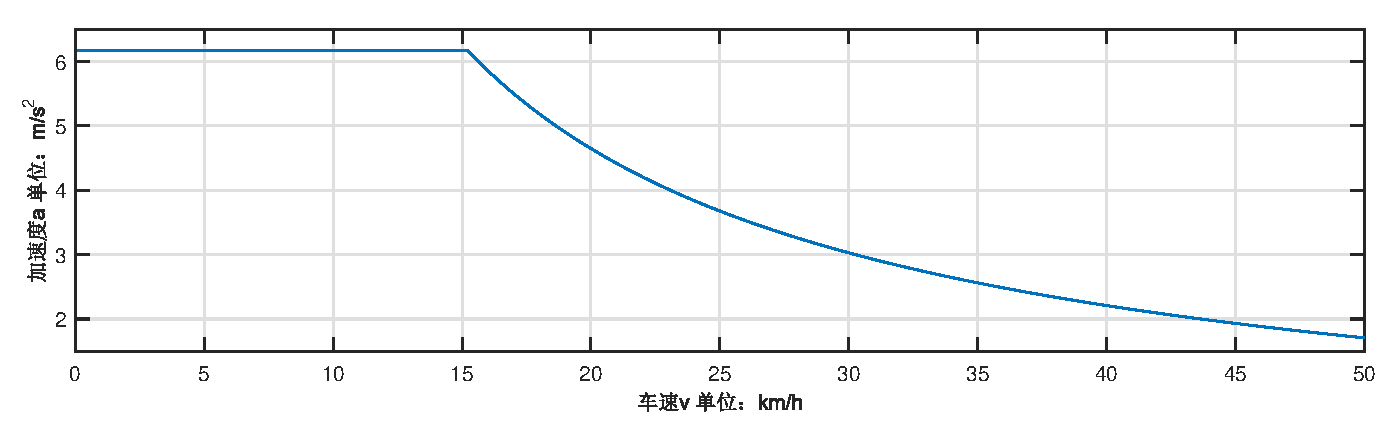
\includegraphics[width=0.9\textwidth]{figures/a-v.eps}
	\caption{车辆的加速度$a$与车速$v$关系}\label{fig:a-v}
\end{figure}

将其转化为车辆的加速度的倒数$\frac{1}{a}$与车速$v$关系图,如图 \ref{fig:aa-v}。

\begin{figure}
	\centering
	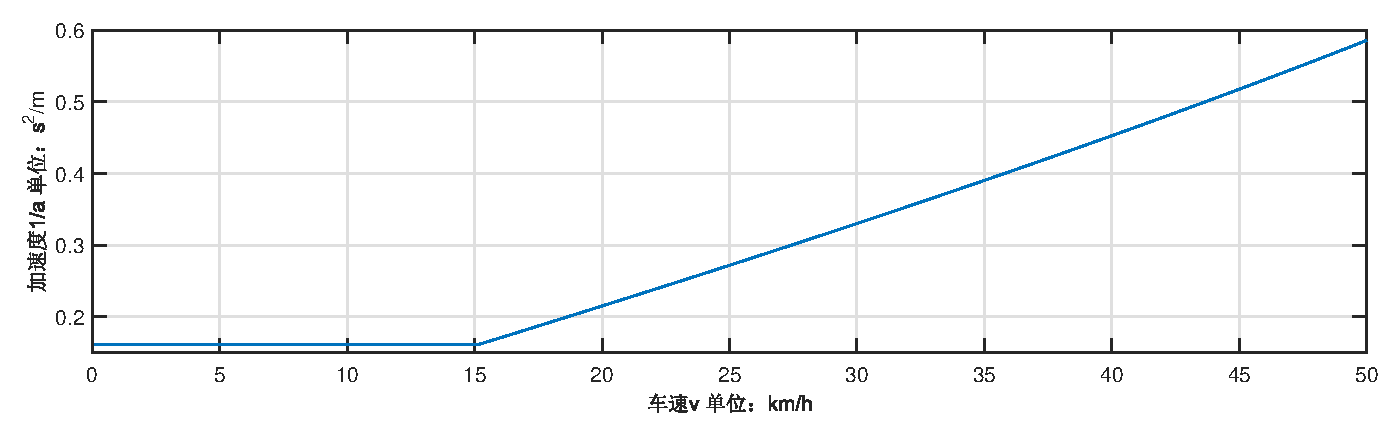
\includegraphics[width=0.9\textwidth]{figures/aa-v.eps}
	\caption{车辆的加速度的倒数$\frac{1}{a}$与车速$v$关系}\label{fig:aa-v}
\end{figure}

计算其对于 x 轴积分即可得到加速度时间值,根据计算,当车辆满足 0$\sim$50km/h 加速时间小于 15 秒时,电池箱的输出功率为 $P_{e3}=68.5 kWh$。

根据以上的计算结果 $P_e=max(P_{e1},P_{e2},P_{e3})=P_{e1}=68.89 kW$,可以满足最高车速超过 150 km/h 的行驶需求。每块电池的额定放电倍率为 6C,则每块电池的额定功率为 $P_0=U_0I_0=3.65 \times 6 \times 37 =810.3 W$,最少需要的电池单体块数为:

\begin{equation}
	n_1=\frac{68.89\times 1000}{810.3}\approx 86
\end{equation}

\subsection{电池包容量计算}
电池包的容量是反映电池系统能够储存多少电能的参数,是电池系统最重要的参数之一,在设计时,电池包的容量参数决定了电池系统有多少块电池单体组成。
电池包的容量要求主要来自于车辆的行驶里程需求,根据目前市面上常见的混合动力汽车的参数列表,如表 \ref{tab:car_group} 和图 \ref{fig:car_group}。可以看到,大部分车型的纯电动里程在 40-59 km 之间,为了保证汽车的纯电动里程符合使用要求,本文将预期的电动车续航里程确定为 60 km。

\begin{table}
	\centering
	\caption{不同品牌的混合动力汽车参数}\label{tab:car_group}
	\begin{tabular*}{0.9\textwidth}{@{\extracolsep{\fill}}ccc}
		\toprule
		厂家			&车型                   &纯电动里程		 \\
		\midrule
		通用	        &Chevy Volt             &85        \\
		宝马		    &i8                     &23 \\
		奥迪            &A1 E-tron              &50         \\
		奥迪            &A3 Sportback E-tron    &27            \\
		保时捷          &Panamera S E-hybrid    &26            \\
		福特            &C-MAX Energi           &31           \\
		福特            &Fusion Energi          &34         \\
		现代            &Sonata PHEV            &43         \\
		现代            &Ioniq PHEV             &47          \\
		凯迪拉克        &ELR                    &58          \\
		凯迪拉克        &CT6 PHEV               &50          \\
		丰田            &Prius Prime            &40      \\
		本田            &Clarity PHEV           &76      \\
		克莱斯勒        &Pacifica Hybrid        &53       \\
		沃尔沃          &XC90 AWD T8 PHEV       &27       \\
		起亚            &Niro PHEV              &42      \\
		起亚            &Optima PHEV            &47      \\
		\bottomrule
	\end{tabular*}
\end{table}

\begin{figure}
	\centering
	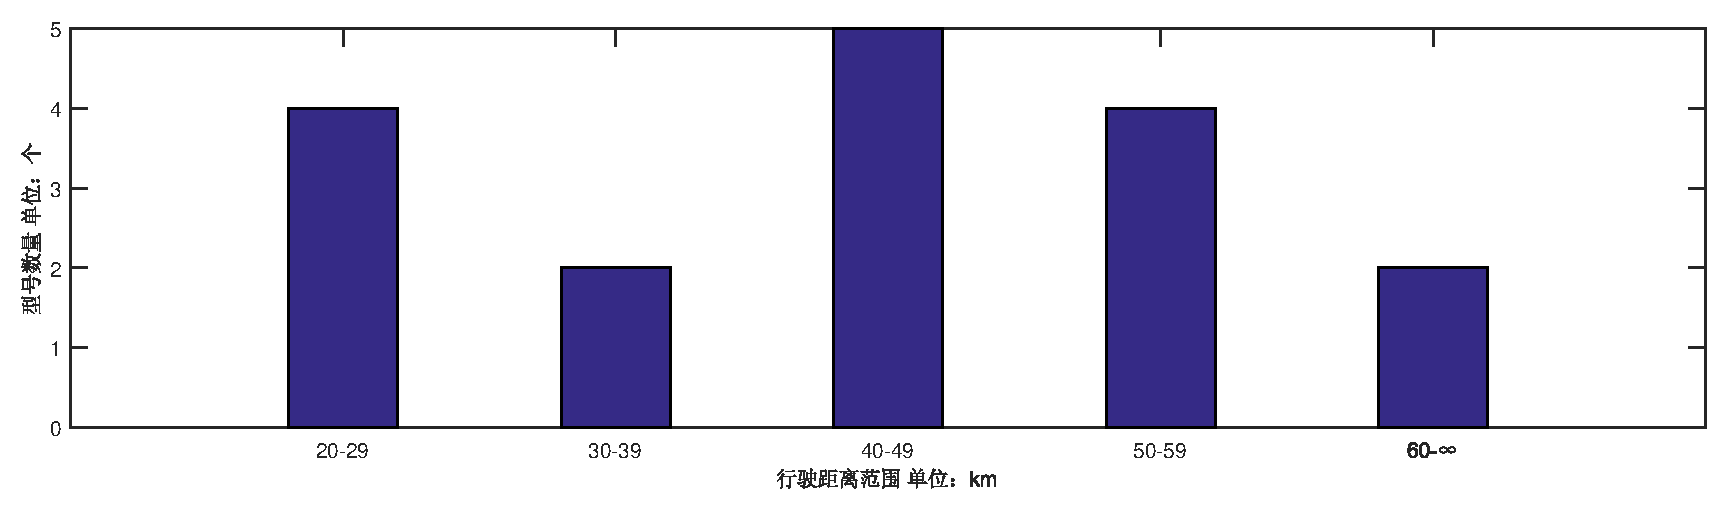
\includegraphics[width=0.9\textwidth]{figures/car_group.eps}
	\caption{不同续航里程区间车型数量}\label{fig:car_group}
\end{figure}

电动车的能量消耗计算时所使用的测试环境是根据中国的典型道路工况决定 \cite{刘希玲2000我国城市汽车行驶工况调查研究},根据《电动汽车能量消耗率和续驶里程试验方法(GB/T 18386-2017)》 标准中规定的 NEDC 工况进行相关的理论计算 \cite{叶磊2012基于中国典型城市循环工况的动力电池测试评价方法},NEDC 工况的速度与时间的关系图如图 \ref{fig:NEDCv},加速度与时间的关系如图 \ref{fig:NEDCa} \cite{kim2009model}。根据 NEDC 工况的速度与加速度数据,和上述车辆的功率平衡方程 \ref{equ:powerequ} ,化简得到式 \ref{equ:powerequ2}。

\begin{figure}
	\centering
	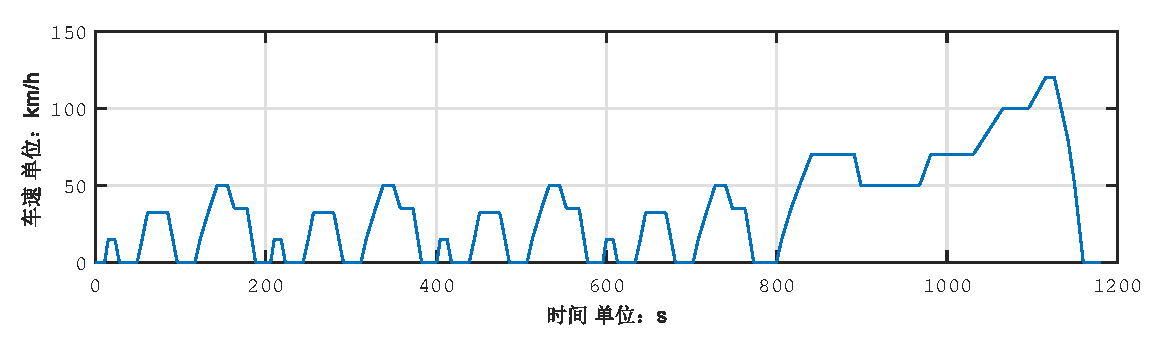
\includegraphics[width=0.9\textwidth]{figures/NEDCv.eps}
	\caption{NEDC 工况速度-时间分布图}\label{fig:NEDCv}
\end{figure}

\begin{figure}
	\centering
	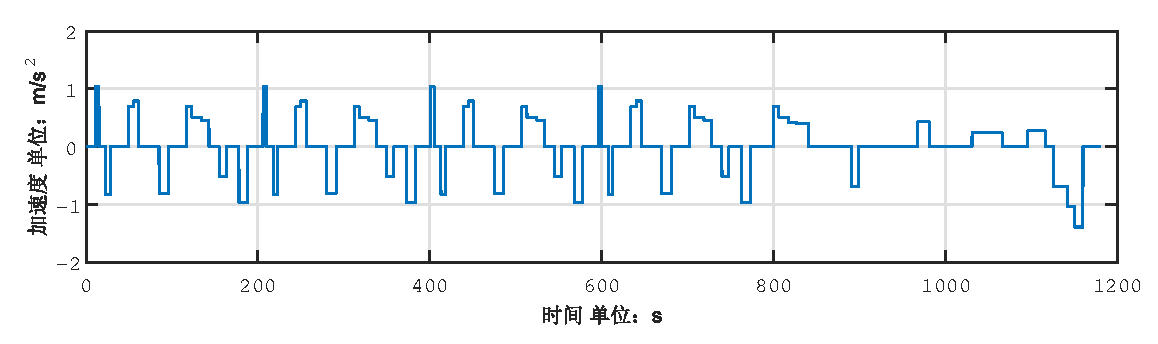
\includegraphics[width=0.9\textwidth]{figures/NEDCa.eps}
	\caption{NEDC 工况加速度-时间分布图}\label{fig:NEDCa}
\end{figure}

\begin{equation}
	\label{equ:powerequ2}
	\eta_T\eta_EP_e=\frac{Gfv_a}{3600}+\frac{C_DAv_a^3}{76140}+\frac{\delta mv_a}{3600}\frac{\mathrm{d}v}{\mathrm{d}t}
\end{equation}

式中的 $P_e$ 为平衡状态的发动机输入功率,$G$ 为匹配所选车辆的自身重量(满载),$f$ 为车辆的滚动摩擦力,$v_a$ 为车辆的运行车速,$C_D$ 为空气阻力系数,$A$ 为迎风面积,$\delta$ 为轿车旋转质量换算系数。

通过计算得出中国典型道路工况功率图(含制动再生)和能量的消耗图 \cite{高建平2015插电式混合动力汽车车载复合电源功率分配策略研究},分别如图 \ref{fig:NEDCp},图 \ref{fig:NEDCe}。
\begin{figure}
 \centering
 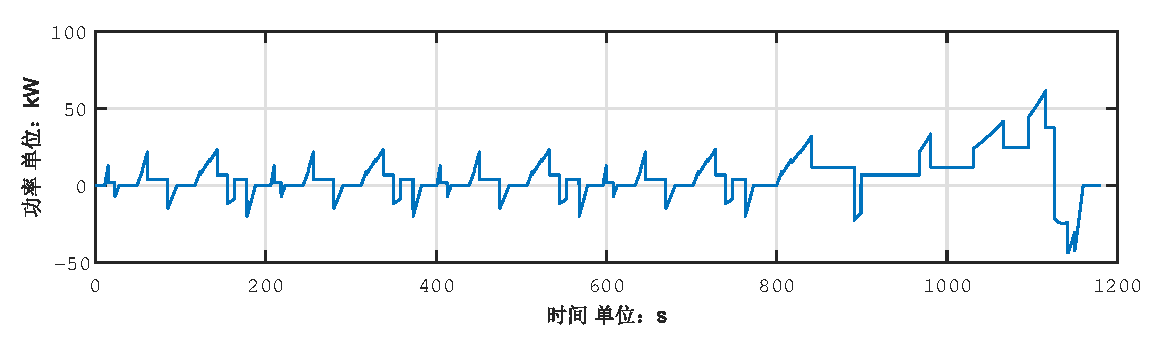
\includegraphics[width=0.9\textwidth]{figures/NEDCp.eps}
 \caption{NEDC 工况功率-时间分布图}\label{fig:NEDCp}
\end{figure}

\begin{figure}
 \centering
 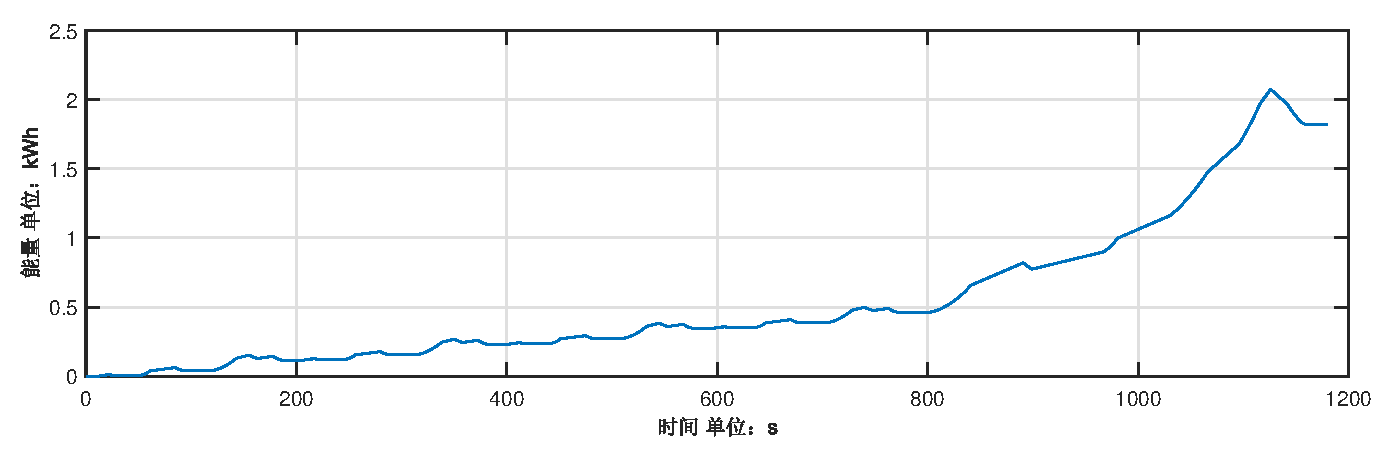
\includegraphics[width=0.9\textwidth]{figures/NEDCe.eps}
 \caption{NEDC 工况能量消耗-时间分布图}\label{fig:NEDCe}
\end{figure}

NEDC 循环工况的总路程为 11.022 km,根据上述计算结果,完成一次 NDEC 循环,该车型需要消耗 1.823 kWh 能量,等效百公里的平均能量消耗为 16.540 kWh。60 公里的里程理论需要 9.924 kWh 的蓄电池能量,等同于电池单体块数:

\begin{equation}
	n_2=\frac{9.924\times 1000}{3.65 \times 37}=73 < 86
\end{equation}

根据能量计算和功率计算得到的电池单体块数限制,可以得到,最终的电池组中的电池单体的数量不应少于 86 块。而电动汽车的电压平台受到了电机控制器和电机额定电压的限制,一般的电动汽车的高压平台电压在 300 至 500 伏之间,在本文的设计中,为了便于电池包的模组设计,故选择 88 个电池单体构成电池系统,并将其分成 8 个模组,每个模组含有 11 个电池单体,电池箱的总额定电压为 321.2 伏。

根据本文最终的设计,可以计算得到电池箱的理论参数,如表 \ref{tab:box}。

\begin{table}
	\centering
	\caption{设计的电池箱理论参数} \label{tab:box}
	\begin{tabular*}{0.9\textwidth}{@{\extracolsep{\fill}}cc}
		\toprule
		参数项目			&数值		 \\
		\midrule
		电池块数/块	     &88  \\
		额定能量/kWh     &11.884  \\
		额定功率/kW      &71.306  \\
		额定内阻/$\Omega$ &1.584  \\
		续航里程/km      &71.852  \\
        最高车速/(km/h)  &152   \\
		\bottomrule
	\end{tabular*}
\end{table}

\section{整车仿真}

上述的理论计算过程得到了电池箱相关的理论参数,为了验证参数的有效性和准确性,本文使用了 AVL Cruise(下称 Cruise)软件,该软件内置一些数据求解器,可以根据输入的整车参数和车辆传动模型,在各种模拟的工况条件下进行测试,并取得模拟车辆的测试结果。Cruise 软件中,模拟车辆的模型采用可视化模块界面,使用者可以很方便的通过使用软件提供的车辆各个组件,修改它们的参数,或者相互组合。并且 Cruise 软件内部内置了丰富的工况模型,例如 NEDC 和 FTP 75 工况,大大简化了在普通车辆计算中的繁琐的工况信息输入过程。

\subsection{整车信息输入}

在使用 Cruise 软件搭建相关的车辆参数模型时,要首先输入车型的整车信息,包括车辆的重量,迎风面积,轴距和轮距等信息,在这里,本文仿真过程中,在 Cruise 软件内输入的相关整车信息如表 \ref{tab:carinfo} 所示。

\begin{table}
	\centering
	\caption{在 Cruise 软件内设置的整车参数} \label{tab:carinfo}
	\begin{tabular*}{0.9\textwidth}{@{\extracolsep{\fill}}cc}
		\toprule
		参数项目			&数值		 \\
		\midrule
		Curb Weight(整备质量)/kg	     &1540  \\
		Gross Weight(满载质量)/kg     &2020  \\
		Frontal Area(迎风面积)/$m^2$      &2.6667\\
		Drag Coefficient(空气阻力系数)     &0.35  \\
		\bottomrule
	\end{tabular*}
\end{table}

在输入完成整车信息之后,还应该设置车辆的驾驶阻力模型,在仿真过程中,车辆阻力是一个至关重要的参数,特别是进行有关车辆的能量消耗和油耗等方面的仿真方面,该参数的模型准确性对于仿真结果影响巨大。该参数在之前的电池包理论计算中被分为四项,分别为滚动阻力,加速阻力,坡道阻力和空气阻力,具体信息参见式 \ref{equ:powerequ}。在 Cruise 软件中,阻力模型被分为若干种阻力模型,车辆物理模型,一阶线性模型(速度),二阶线性模型(速度和速度平方),本文在理论计算的过程中使用的模型为物理模型,该模型下车辆的阻力模型与车辆的空气阻力和车辆轮胎的滚动阻力有关。

\subsection{组建车辆动力模型}

当完成了车辆的整车信息输入之后,接下来是要完成对于车辆的动力模型的构建,本文选用的模型为串联式混合动力模型,搭建的模型的结构如图 \ref{fig:car_structure} 所示。其中,设置的主减速比为 6.058(根据电机的最高转速和车辆的轮胎滚动半径计算得到),主减速器的机械效率为 $96\%$,差速器的效率设定为理想值 $100\%$,总传动链的机械效率为 $96\%$,与理论计算时的机械效率保持一致。

\begin{figure}
	\centering
	\includegraphics[width=0.75\textwidth]{figures/car_structure_cruise.png}
	\caption{Cruise 车辆动力模型}\label{fig:car_structure}
\end{figure}

在车辆运行时轮胎的滚动阻力系数与车速有关,由于轮胎与地面间存在振动,随着车辆的行驶车速上升,轮胎的响应振动频率随之上升,当到达某一定值时轮胎的表面会发生驻波现象,轮胎的外边缘会变成波浪状,造成阻力系数剧烈提升。而轮胎的滚动阻力系数与多种因素有关,包括轮胎的充气压力,轮胎的帘线类型,轮胎的橡胶种类有关。该仿真车辆轮胎的滚动阻力系数特性曲线参见图 \ref{fig:tier_characteristics}。

\begin{figure}
	\centering
	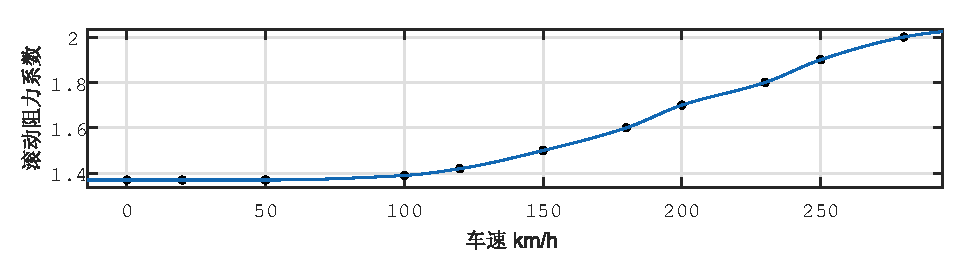
\includegraphics[width=0.9\textwidth]{figures/tier_characteristics_cruise.eps}
	\caption{仿真中的轮胎滚动阻力特性曲线}\label{fig:tier_characteristics}
\end{figure}

\subsection{电动机参数设定}
在本次仿真过程中,使用的电动机模型为软件自带的电动机模型,电机类型为异步电动机,额定电压设定为 320V,最高转速为 10000 rpm,该电机的万有特性曲线如图 \ref{fig:asm_characteristics} 所示。

\begin{figure}
	\centering
	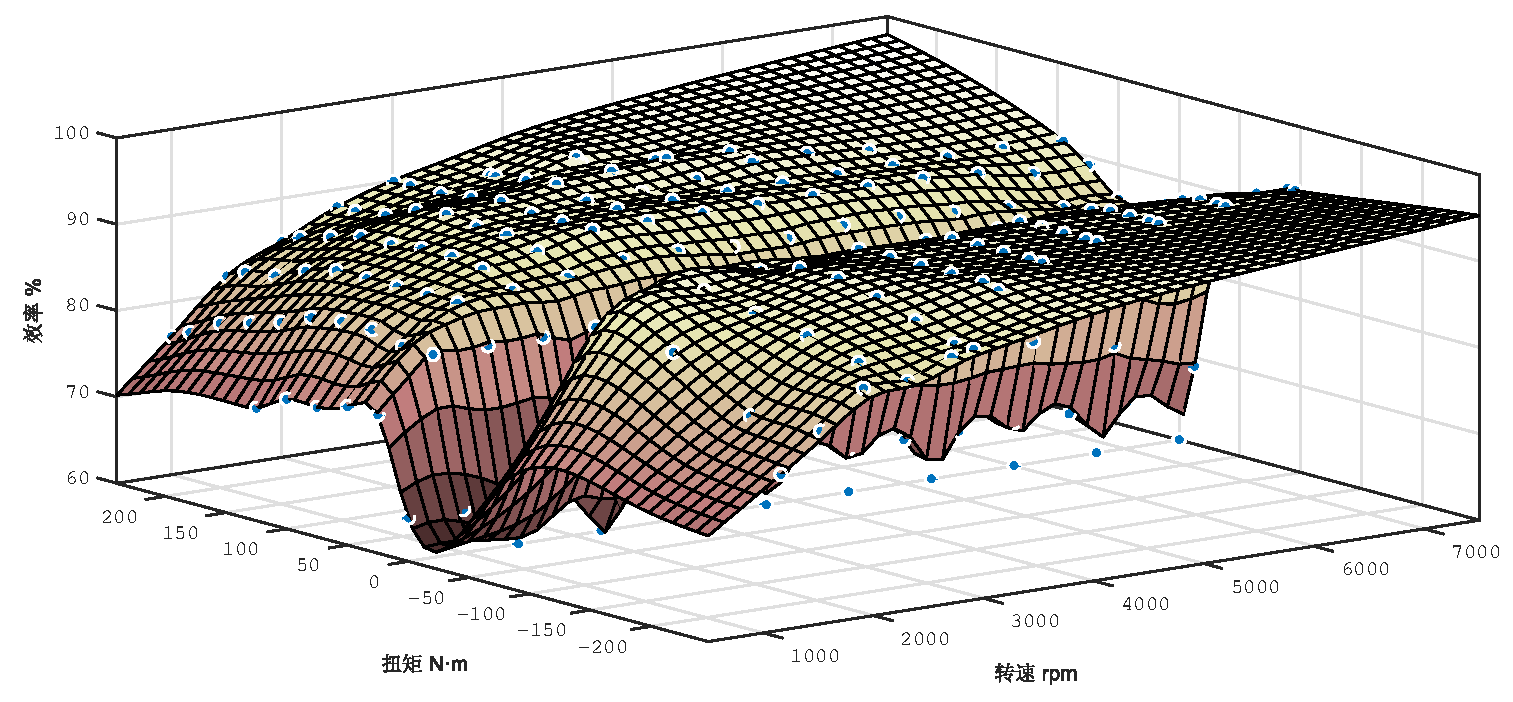
\includegraphics[width=0.9\textwidth]{figures/asm_characteristics_cruise.eps}
	\caption{电机的万有特性曲线}\label{fig:asm_characteristics}
\end{figure}

在之前的理论计算中,本文使用的电机效率为该电机万有特性曲线获得的平均值 $85\%$。

\subsection{电池箱参数设定}
接下来进行的是电池箱参数的设定,电池箱设定的参数根据厂家提供的电池单体信息和本文设计的参数,其中电池单体参数参见表 \ref{tab:cell} 所示数据。而电池的 OCV-SOC 曲线为实验室测的的数据,如表 \ref{fig:cell-OCV} 所示。

\begin{figure}
	\centering
	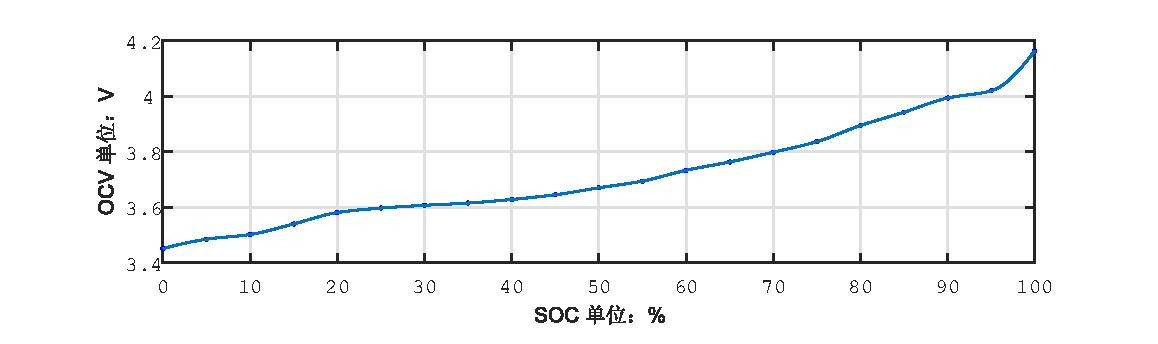
\includegraphics[width=0.9\textwidth]{figures/cell-OCV.eps}
	\caption{LP2714897 电池单体 OCV-SOC 特性曲线(实验获得)}\label{fig:cell-OCV}
\end{figure}

根据上述匹配的结果,输入对应的电池连接方式,为 88 个电池单体串联的方式进行连接。

\subsection{仿真工况与驾驶员设定}
Cruise 软件自带了许多工况信息,本文使用了其中预置的 NEDC 工况,该工况的信息见图 \ref{fig:NEDCv}。在仿真过程中使用的模型是车辆的物理运动模型,车辆为满载状态下的情况。驾驶员驾驶习惯状态如表 \ref{tab:driver} 所示。当仿真开始时,电池箱的 SOC 值被设定为 $100\%$。

\begin{table}
	\centering
	\caption{Cruise 驾驶员习惯} \label{tab:driver}
	\begin{tabular*}{0.9\textwidth}{@{\extracolsep{\fill}}cc}
		\toprule
		参数项目			&数值		 \\
		\midrule
		Starting Speed(开环起步转速)/rpm	     &4000     \\
		Customer Starting Speed(闭环起步转速)/rpm &1200  \\
		Maximum Brake Force(最大刹车踏板力)/N      &10   \\
		Foresight Time(前瞻时间)/s      & 0.25      \\
		\bottomrule
	\end{tabular*}
\end{table}

\subsection{Cruise 仿真结果}
软件仿真后的结果被分为数类,其中包括了车辆的运动参数,车辆的电池箱参数,车辆的驾驶员姿态参数,道路参数。其中,本文只对于电池箱的有关参数进行分析,在行驶的整个过程中,电池箱有关参数的变化如图 \ref{fig:result} 所示。

\begin{figure}
	\centering
    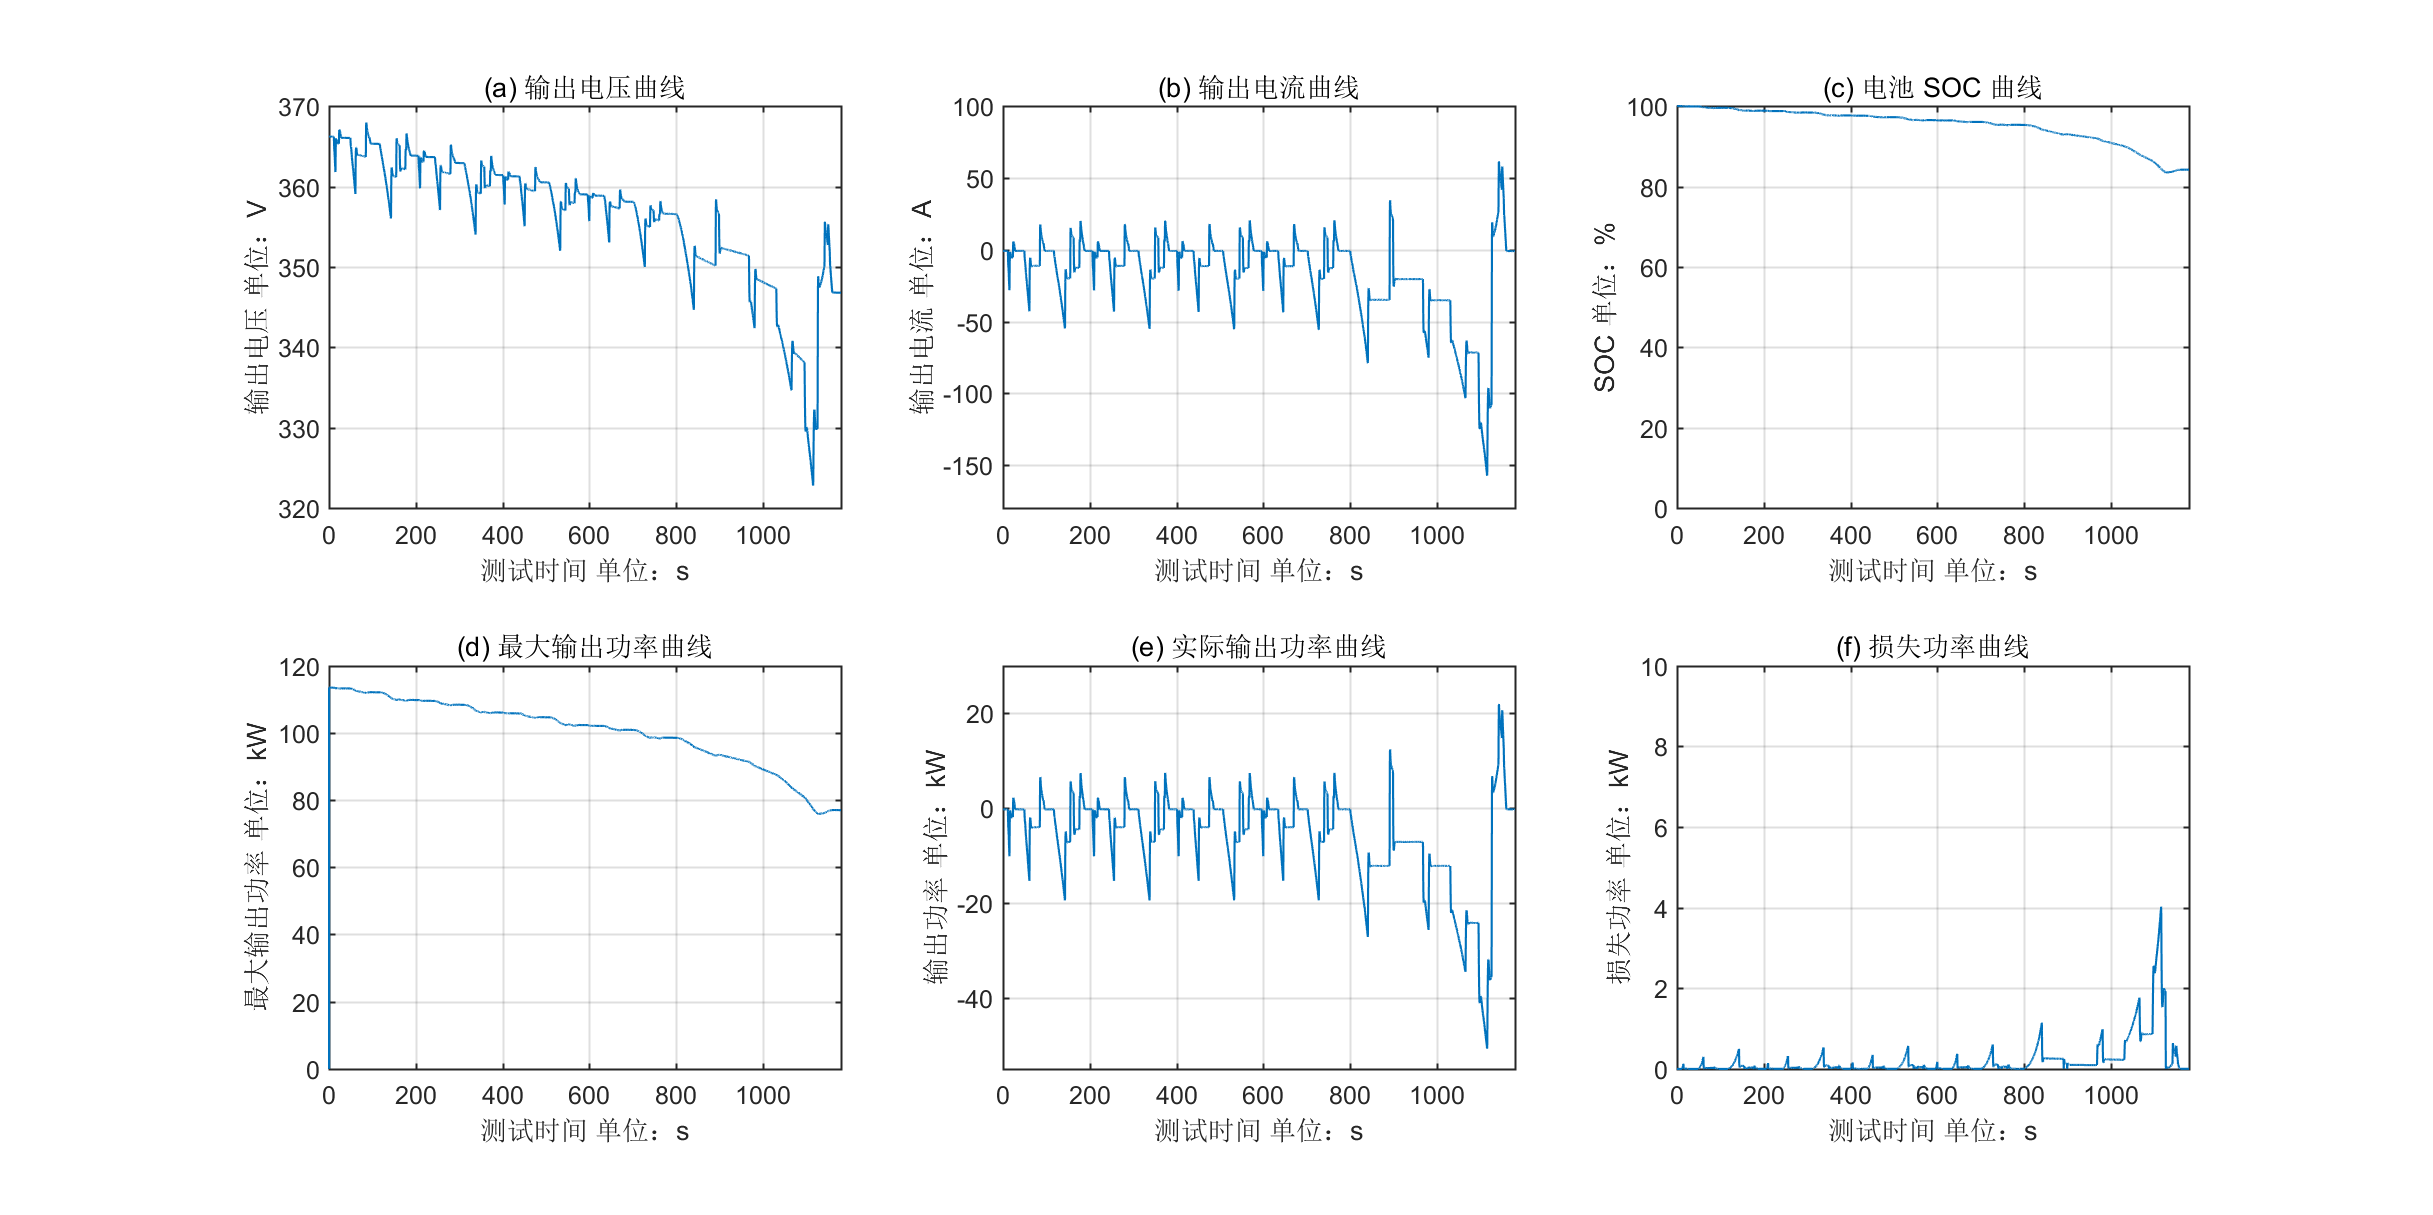
\includegraphics[width=1\textwidth]{figures/result.eps}
	\caption{Cruise 仿真结果}\label{fig:result}
\end{figure}

可以看出,仿真的过程中,电池箱未发生功率不足的情况,电池箱的最大输出功率始终超过电池箱的输出功率,这证明了电池箱在输出功率方面符合了要求,电池箱的功率计算有效。在完成了一次 NEDC 的循环后,电池箱的剩余电量为 31.1477 Ah,消耗的电量为 5.8523 Ah。根据仿真结果,计算总计的续航里程为 $S_D=\frac{37 \times 11.022}{5.8523} = 70.035 km$,与通过理论计算得到的(参见表 \ref{tab:box})数据基本一致,仿真结果与理论计算的相对误差为 $2.6\%$,可以认为理论计算的结果具有有效性,并且比较准确。

\section{理论计算误差分析}
关于上述理论计算的过程中存在的误差,下文将误差因素进行了一个总结,并且对于弥补误差,获得更精确的理论计算值提供了一个方法,希望能供后续的研究参考,并且改进计算模型。实验误差的种类分为系统误差和随机误差,但是由于该计算过程仅仅使用计算机模拟仿真,各个参数对于结果的影响均包含在系统计算范围之内,可以人为进行控制,故可以认为仿真的测量值不存在随机误差。所以下文的误差分析仅仅针对于系统存在的误差进行分析。

\subsection{电池参数误差}

\subsubsection{电压误差}
厂家提供的电池单体参数,参见表 \ref{tab:cell},对于电池的额定电压,在参与理论计算的计算过程中被当做一个固定不变的值,本文对于电池容量的计算也仅仅通过对于额定电压和安时数进行简单的相乘计算,而在实际情况下,电池的输出电压是一个和电池电量相关的数值,在实验室数据中,随着电池的放电,电池的电量下降,电池的开路电压(OCV)也随之发生了改变,如图 \ref{fig:cell_deviat} 所示,实验室数据和理论计算时使用的数值有偏差。因为上述理论计算过程中采用的容量计算方式是根据电池安时和电池的额定电压数据进行计算的,故当电池的开路电压发生了改变,电池的容量估计便存在误差,对于计算结果产生了影响。

\begin{figure}
	\centering
	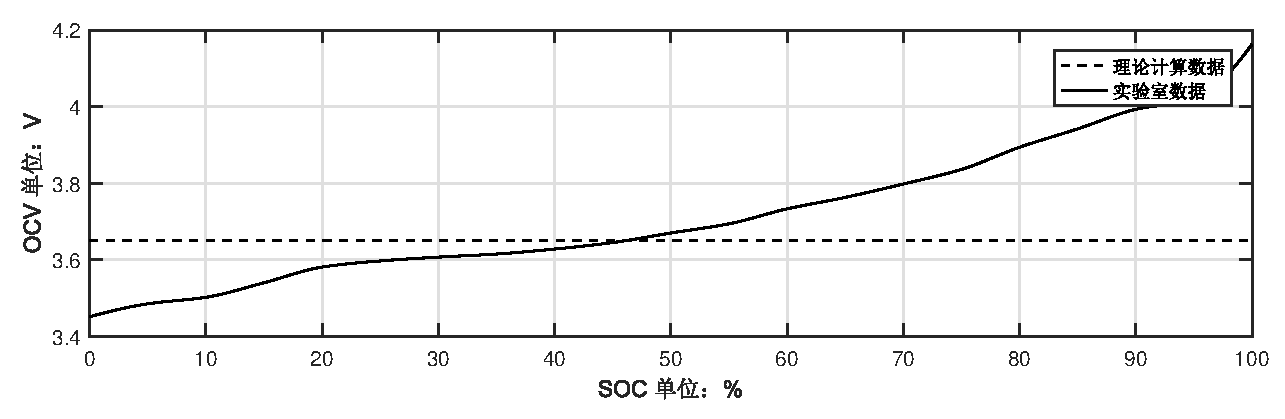
\includegraphics[width=0.9\textwidth]{figures/cell_deviat.eps}
	\caption{电池单体的 OCV 计算偏差}\label{fig:cell_deviat}
\end{figure}

这也就是说在理论计算的过程中,电池的电压模型建模不够精确,如果想要更加精确的计算结果,可以在系统中输入电池的 OCV-SOC 曲线,根据电池的 OCV 曲线,结合安时计测量,获得电池的准确电量值。该值不仅仅对于电池的的容量有影响,可以看出,在仿真曲线的后期,由于 SOC 的下降,电池的开路电压下降,导致电池包的输出电压大幅度下降,而由于车辆的阻力和车速未发生变化,维持车辆所需要的输出功率并没有发生改变,导致电池包的输出电流剧烈上升。在这种情况下,电池包的总输出电流会超过理论计算中的值,造成线路承受巨大的电流,有安全风险。

\subsubsection{内阻误差}
在本文的理论计算章节,忽略了电池内阻的影响,而在理论仿真的过程中,对于内阻的设置,也仅仅设置了一个固定的内阻值,而在实际的使用当中,内阻对于电池放电的影响十分重大,不可忽视。首先,在电池的能量计算中,电池输出的能量多少与内阻的高低相关,由于电池采用安时计算的方式计算能量,在电池放电或充电的过程中,电池内阻会消耗电能,并产生焦耳热 $I^2R \delta t$,可以看到,焦耳热的多少与电流的平方成正比,故在大倍率、高电流的放电情况下,电池的内阻产生的焦耳热会大大增加。根据研究结果,电池的内阻是一个与电池的 SOC 以及温度息息相关的的值,当电池的 SOC 下降的情况下,电池的内阻值会逐渐上升,而在温度较低的环境下电池的内阻也会显著上升,电池内阻会影响电池的容量 \cite{刘伟2016锂离子动力电池直流内阻测试及其应用研究}。其次,电池的输出功率与电池的内阻有关,当电池的内阻为 $\gamma$ 时,电池理论上无法输出超过 $\frac{U_ocv}{\gamma}$ 的功率。相比纯电动汽车,混合动力汽车中搭载的电池单体数量较少,在相同的功率需求条件下,电池的充放电倍率较大,电池内阻过大会导致电池输出功率不足,在车辆需要大功率输出的时候,电池不仅无法提供足够的输出功率,还会产生电池过放的风险,使电池处于不安全状态。

在理论计算中,可以先在实验室内控制环境条件,譬如气温的高低。在不同的 SOC 以及温度条件下测量电池的内阻值,并建立电池的内阻模型,根据电池的 SOC 情况使用不同的内阻值,一般情况下,电池的 SOC 值越低,电池的内阻就会相应的有所提高,电池箱的放电倍率越大,电池的内阻上升越快 \cite{罗玉涛2016延长锂离子电池寿命的电动汽车复合电源设计};并计算电池的内阻产生的热量,对于电池的温度模型进行建模仿真,仿真出电池包在运行的时刻的不同温度条件下的内阻情况,将两种因素(温度以及 SOC)同时带入能量计算的过程,可以获得更加精准的电池能量输出量,这会对于车辆的行驶里程等容量相关的计算结果更加精确可靠,并且可以验证电池包的输出功率是否能够满足使用要求。

\subsection{电机参数误差}

本文理论计算中有关电机的参数仅有电机的效率参与了计算,而在实际的仿真中,是使用了电机的万有特性曲线进行效率的计算,这之间的不同就涉及到了电机效率参数的误差。

电动机类似于内燃机,在实际的工作情况下,其工作效率同样受到其转速和负载转矩的影响,但普通的特性曲线仅仅只能表示两种参数之间的关系,而不能表示三种参数的相关关系,于是电动机也存在万有特性曲线。电动机的万有特性曲线的横坐标为电动机的转速和负载转矩,纵坐标为电动机的能量转换效率。在理论计算过程中,本文使用了平均的电机的能量转换效率,即为 $85\%$。但是在实际的情况下,电机的能量转换效率在不同的车速情况下,也会发生变化,如图 \ref{fig:asm_characteristics} 所示。此误差会导致理论计算的时候,电池箱的功率与实际的输出值不符合,存在一定的误差。

可以在计算的时候,在每一时刻的情况下,根据车速和车辆的加速度状态,与车辆的主减速器,计算出车辆的每一时刻的电机的负载转矩和转速。根据这两个因素计算电动机的能量转换效率,并参与电动机的输出功率的计算,使用这种方法得到的输出功率曲线才是更加精确的理论值。

\subsection{车辆动力模型参数误差}
在计算的过程中,本文使用的车辆动力模型是依照纯物理模型建立的模型,是根据汽车的车速,加速度计算的。但是在实际情况下,汽车的阻力模型是一个与许多因素有关的复杂的模型,不仅仅与外部环境譬如温度,路面不平度,路面的摩擦系数,空气密度,风阻有关,也与车辆的结构有关,譬如车辆的空气动力学模型,车辆的轮胎刚度,车辆的悬架刚度等等因素有关。当然在计算的过程中,考虑到所有的因素是不可能的,但是可以通过一系列的矫正系数,来使本文的计算结果更加逼近实际测量值,但是这需要大量的实验数据作为基础。

在计算的过程中,本文忽视了各种动力系数的变化,在车辆进行低速到高速的变速运行的情况下,车辆的空气阻力系数,轮胎滚动阻力系数也会发生改变,可以测量车辆的各项参数在不同车速条件下的值,并对于计算结果进行校正;在车辆的传动链上,差速器和减速器也会根据车速的不同,产生机械转换效率的改变,如果想要更加精准的测量值,可以根据各个部件的这种改变也可以在后续的改良计算中进行改良,来获取更加精确的效率系数。

在本文的理论计算中,对于旋转质量系数的计算公式是采用经验计算公式确定的,如式 \ref{equ:rot},但是该计算公式在车辆的质量,车辆的传动结构发生差异也会产生差异,如果想要更加精确地结果可以根据指定车辆的结构计算此系数,会使结果更加精确。

在设计电池系统参数的时候,设计完成的参数应用于电池箱之后,一旦电池系统参数发生改变,同样会改变电池箱的物理参数,例如根据电池箱的参数大小决定电池箱内部使用多少块电池单体,这会导致电池箱的大小和质量等等参数发生。因为电池箱是安装在车辆上的部件,电池箱的质量会影响车辆的物理特性,包括车辆的轴荷状态和车辆的阻力等相关系数。也就是说在设计完成后,电池箱的参数会反而影响所匹配的车辆的运行状态。在理论计算中,本文将车辆的质量固定为满载状态,不受电池箱的质量影响,而在实际的应用当中,电池箱由于质量较大,其参数对于车辆的影响同样较大,故如果想要获得更加精确的车辆阻力模型需要在理论计算环节考虑到电池箱参数对于车辆整体的动力学模型的影响。

